\section{Dynamics Discretization and Stability}
\subsection{Motivation}
即使有了上节所述的连续时间系统状态方程，我们依旧无法在计算机得到$x(t)$，也就无法根据此进行计算机控制。本节将介绍如何把连续的ODE方程转换成离散的数值积分形式并在实际的计算机硬件中实现。理想上，我们期望通过对离散化的状态方程数值积分后可以得到和实际物理系统一样的结果，且应该是low-cost的。相较于连续时间的状态方程，离散状态方程是更加general的，能表达更多东西，因为在现实中有许多量根本不是连续的。如，在某个时刻突然出现的一个外部扰动。
\begin{itemize}
    \item In general, we can't directly solve $\dot x=f(x)$ for $x(t)$, because most $f(x)$ are nonlinear, but we can just handle linear ODE.
    \item In terms of numerical computation, we need to represent $x(t)$ with discrete values.
    \item Discrete-time models can capture some effects that continuous ODEs can't. For example, discontinuous change of force during contact.
\end{itemize}
\subsection{``Explicit'' Form}
首先讨论显式（explicit form）的离散时间系统方程，这意味着系统的下一个状态可以直接表达成当前状态与输入的显函数，进行数值积分的时候不用解求根方程。
\begin{equation}
    x_{k+1} = f_d(x_{k}, u_{k})
\end{equation}
\subsubsection{Simplest Discretization: Forward Euler Integration}
\begin{equation}
    x_{k+1} = \underset{f_d(x_k)}{\underbrace{x_k + hf_d(x_{k}, u_{k})}}
    \label{equ:pen_fel}
\end{equation}
\begin{itemize}
    \item Pendulum Simulation
          Let $l=m=1$,
          \begin{figure}[H]
              \centering
              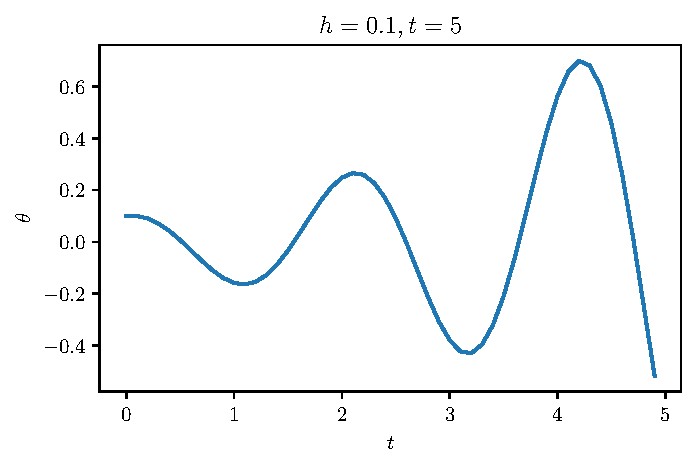
\includegraphics[scale=.75]{./tex/ch2/1.pdf}
              \caption{Simulation parameters: $h=0.1, t=5$}
          \end{figure}
          \begin{figure}[H]
              \centering
              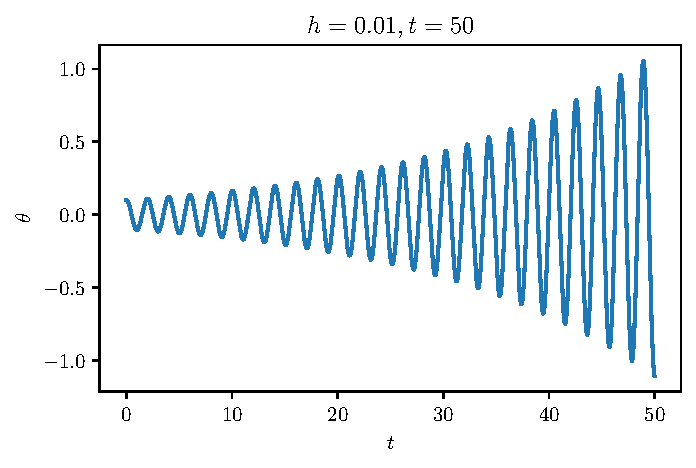
\includegraphics[scale=.75]{./tex/ch2/2.pdf}
              \caption{Simulation parameters: $h=0.01, t=50$}
          \end{figure}
    \item 从欧拉前向积分的结果可以看出，我们取$\theta=0.1,\dot\theta=0$为初始状态 进行数值积分，无论把积分步长取得多小，最终结果居然都是发散的。但是在上个section中，我们分析了在$\theta=0,\dot\theta=0$处的平衡点状态，它是临界稳定的而不是发散的。这在某些情况是很致命的，本来实际稳定的系统在数值积分后就不稳定了，说明这个积分方法在这种情况是不能接受的。
    \item 从连续状态方程来看，单摆的$\dot\theta$是一个$\sin$函数，而用前向欧拉积分法，相当于一直用本时刻的梯度来估计这一段时间的梯度，这在sin函数中意味着会一直高估系统的加速度，会导致系统的能量一直上升。
    \item It is obvious that not matter how small time step $h$ is, the simulation of pendulum dynamics blows up finally. In other words, the discrete system, forward euler integration of pendulum dynamics, is unstable.
\end{itemize}
\subsubsection{Stability of Discrete-Time Systems}
\begin{itemize}
    \item Recall continuous-time systems:
          \begin{align*}
              \text{Re}\left[\text{eig}\left(\frac{\partial f}{\partial x}\right)\right]<0 \Rightarrow \text{stable} \\
              \text{Otherwise} \Rightarrow \text{unstable}
          \end{align*}
    \item In discrete-time system, dynamics is an iterated map:
          \begin{equation}
              x_N = \underset{\text{N times}}{\underbrace{f_d(f_d(f_d(\cdots f_d(x_0))))}}
          \end{equation}
    \item Assuming the equilibria of $f_d$ stays still, we can linearize the dynamics by applying chain rule:
          \begin{equation}
              \frac{\partial x_N}{\partial x_0}=\left.\underset{\text{N times}}{\underbrace{\frac{\partial f_d}{\partial x}\frac{\partial f_d}{\partial x}\frac{\partial f_d}{\partial x}\cdots\frac{\partial f_d}{\partial x}}}\right|_{x_0} = A_d^N
              \text{(not rigorous, why?)}
          \end{equation}
    \item Assuming we setup coordinates so equilibria is at $x = 0$
          \begin{align}
              \text{stable} \Rightarrow & \lim _{k\rightarrow \infty } A_{d}^{k} x_{0} =0\ \forall x_{0} \\
              \Rightarrow               & \lim _{k\rightarrow \infty } A_{d}^{k} =0                      \\
              \Rightarrow               & \left| \text{eig}( A_{d})\right| < 1
          \end{align}
    \item Let's apply this to pendulum forward euler integration, according to Equ. \eqref{equ:pen_fel}
          \begin{equation}
              A_d = \frac{\partial f_d}{\partial x_k} = I + hA = I + h 
              \begin{bmatrix}
                  0                       & 1 \\
                  -\frac{g}{l}\cos \theta & 0
              \end{bmatrix}
          \end{equation}
          We calculate that $\text{eig}\left(\left.A_d\right|_{\theta=0}\right)=1\pm0.31226657i$, when $h=0.1$.
    \item Plot $\left|\text{eig}\left(A_d\right)\right|$ v.s. $h$
          \begin{figure}[ht]
              \centering
              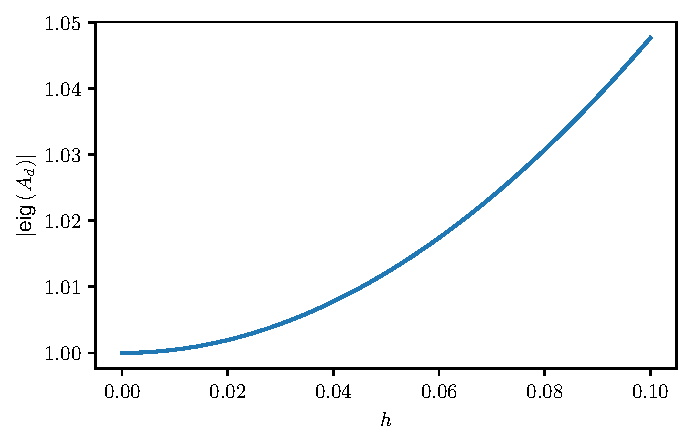
\includegraphics[scale=.75]{./tex/ch2/3.pdf}
              \caption{Relationship between $\left|\text{eig}\left(A_d\right)\right|$ and time step $h$.}
          \end{figure}
          We find that the discrete system is only marginally stable when $h\rightarrow 0$.
    \item Intuition:
          Linear approximation always \textcolor{red}{overshoots} (we'll discuss later) $\sin \theta$:
          \begin{figure}[ht]
              \centering
              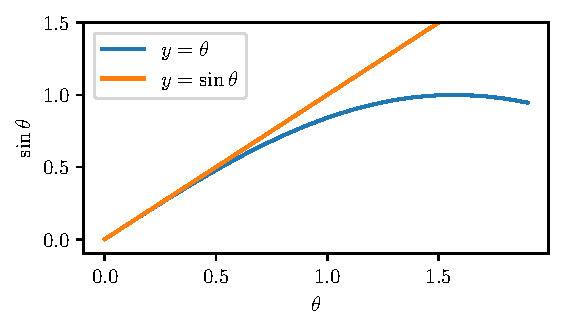
\includegraphics[scale=.75]{./tex/ch2/4.pdf}
              \caption{Linear approximation of $\sin\theta$.}
          \end{figure}
\end{itemize}
\subsubsection{Summary}
\begin{itemize}
    \item Be careful with ODE discretization.
    \item Sanity check based on energy, momentum, behavior (conservation and/or dissipation)
    \item Don't use forward euler integration, although it is commonly used in RL, gym, etc..
    \item 前向欧拉积分总是overestimate系统的加速度，对于有阻尼的系统来说，这可能不会有很严重的影响，但是对于没阻尼的系统（如本节分析的），别用前向欧拉积分
\end{itemize}
\subsection{A better explicit integrator}
\begin{itemize}
    \item $\text{k}^{\text{th}}$ order Runge-Kutta (RK) method (industry standard).
    \item Intuition: Euler fits a line ($\text{1}^{\text{st}}$ order) segment over each time step. RK fits a cubic polynomial, which has much better accuracy.
    \item Pseudo code:
          \begin{equation}
              \begin{aligned}
                  x_{n+1} = & x_{n} +\frac{h}{6}( k_{1} +2k_{2} +2k_{3} +k_{4}) \\
                  k_{1} =   & f( x_{n}, u)                                         \\
                  k_{2} =   & f\left( x_{n} +\frac{h}{2} k_{1}, u\right)           \\
                  k_{3} =   & f\left( x_{n} +\frac{h}{2} k_{2}, u\right)           \\
                  k_{4} =   & f( x_{n} +h k_{3}, u)
              \end{aligned}
          \end{equation}
          RK有很多种形式，取决于中间的knot point怎么选。
          即便RK比前向欧拉效果好，但是显式方法并不适用于所有系统，比如高刚度的机械系统，RK也会爆炸。
          $u$在每个点的具体取值取决于取的控制离散化方法，如果是零阶保持器的形式，那么即如上，但若是一阶保持器，则要把$u$也做插值。
    \item Pendulum Simulation
          Let $l=m=1$,
          \begin{figure}[H]
              \centering
              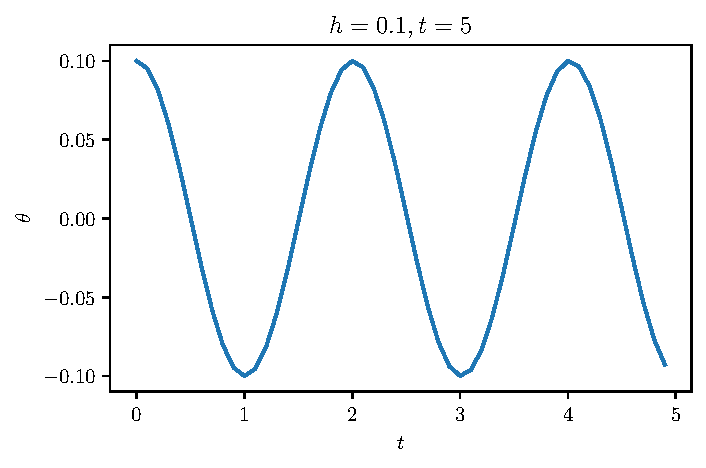
\includegraphics[scale=.75]{./tex/ch2/5.pdf}
              \caption{Simulation parameters: $h=0.1, t=5$}
          \end{figure}
          \begin{figure}[H]
              \centering
              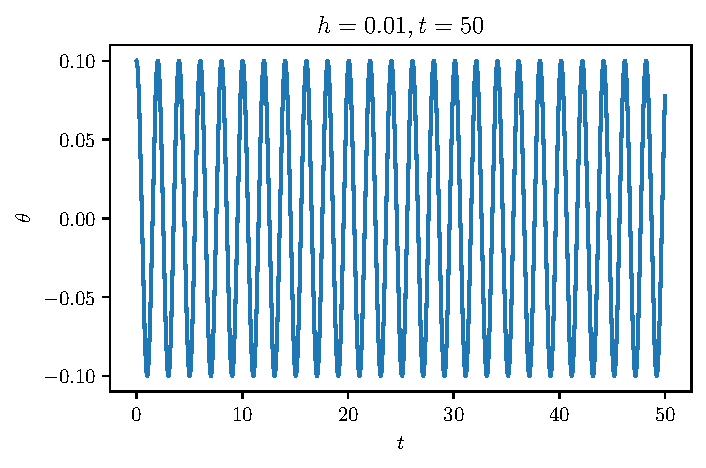
\includegraphics[scale=.75]{./tex/ch2/6.pdf}
              \caption{Simulation parameters: $h=0.01, t=50$}
          \end{figure}
          \begin{figure}[H]
              \centering
              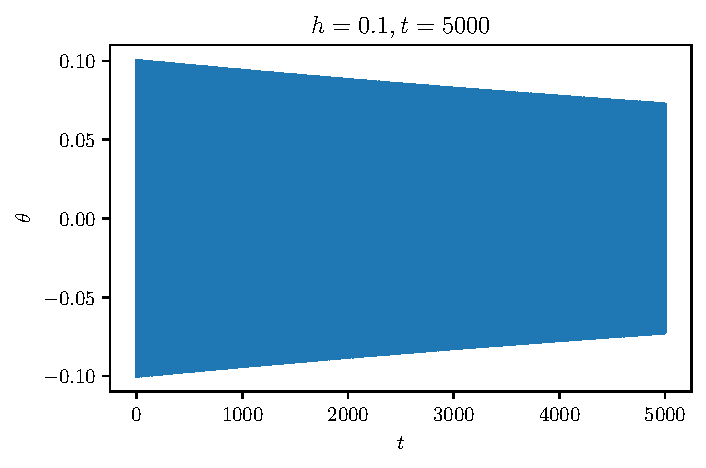
\includegraphics[scale=.75]{./tex/ch2/7.pdf}
              \caption{Simulation parameters: $h=0.1, t=5000$}
          \end{figure}
          - Stability with respect to time step $h$. What matters is the ratio of the natural frequency to the integrator step size.
          \begin{figure}[H]
              \centering
              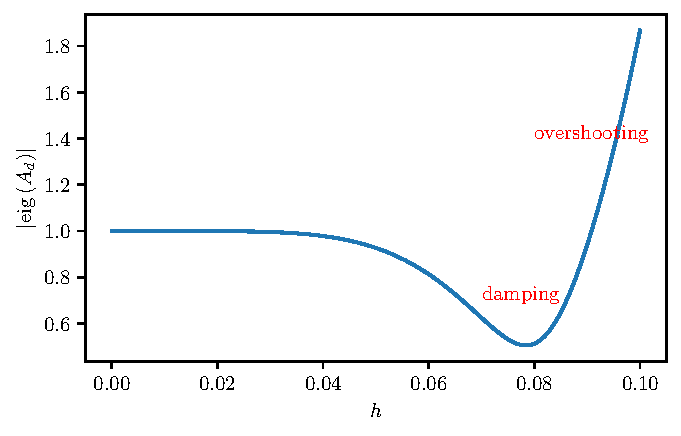
\includegraphics[scale=.75]{./tex/ch2/8.pdf}
              \caption{Relationship between $\left|\text{eig}\left(A_d\right)\right|$ and time step $h$.}
          \end{figure}
    \item Accuracy win weights over additional compute cost.
    \item Even sophisticated integrators have badness, so always remember to do sanity check.
\end{itemize}
\subsection{``Implicit'' form}
\begin{equation}
    f_d(x_{k+1},x_k,u_k)=0 
\end{equation}
\begin{itemize}
    \item Simplest version: Backward Euler Integration
          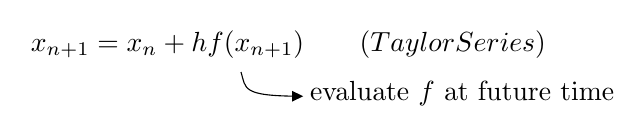
\begin{tikzpicture}[x=0.75pt,y=0.75pt,yscale=-1,xscale=1]
              \draw    (323,34.5) .. controls (325.43,42.43) and (323.15,45.96) .. (350.39,46.16) ;
              \draw [shift={(353,46.17)}, rotate = 180] [fill={rgb, 255:red, 0; green, 0; blue, 0 }  ][line width=0.08]  [draw opacity=0] (5.36,-2.57) -- (0,0) -- (5.36,2.57) -- cycle    ;
              \draw (220.5,13.4) node [anchor=north west][inner sep=0.75pt]    {$x_{n+1} =x_{n} +hf( x_{n+1}) \qquad \text{(Taylor Series)}$};
              \draw (355,37.5) node [anchor=north west][inner sep=0.75pt]   [align=left] {evaluate $\displaystyle f$ at future time};
          \end{tikzpicture}
    \item How do we simulate: solve root-finding problem for $x_{k+1}$
          \begin{equation}
              f_d (x_{k+1}, x_k, u_k) =x_k +hf(x_{k+1}) - x_{k+1}=0
          \end{equation}
    \item Pendulum Simulation
          \begin{figure}[ht]
              \centering
              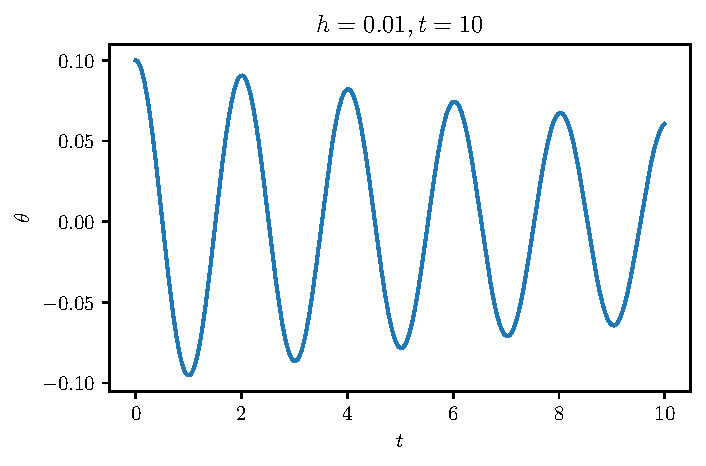
\includegraphics[scale=.75]{./tex/ch2/9.pdf}
              \caption{Pendulum Simulation Using Backward Euler Integration.}
          \end{figure}
    \item Backward Euler Integration owns an opposite energy behavior from Forward Euler Integration, the former damped while the latter blew up. 后向欧拉法倾向于低估系统的加速度，与前向欧拉相反，比前向法更加稳定。后向欧拉法给系统增加了人工的阻尼（artificial damping）
    \item While nonphysical and nasty damping, this effect allows simulators to take big steps and is often convenient, and is very common in low-fidelity simulators in graphics/robotics (PyBullet, Mujoco, etc).
\end{itemize}
\subsection{Other Notes}
\begin{itemize}
    \item Implicit methods are often more stable than explicit methods. However, stable does not mean ``accurate''.
    \item For forward simulation, solving implicit equation can be more expensive.在前向rollout时，这种方法是expensive的
    \item In many direct trajectory optimization methods, they're not more expensive. 但是在非因果的系统（non-casual）中，如在做离线全局轨迹优化问题时，这种方法比较有效
    \item 对于很刚性（stiff）的系统，天生就是难仿真的，因为其中含有许多高频分量，必须取小的步长才能捕获到这些高频分量中的信息
    \item 龙格库塔法是基于4个点来获得状态的近似，当然也可以取很多很多点，理论上可以达到一个任意精度的连续近似。（硕哥指出）。但是这种不一定会更好，一来是算力要求更高，而来是，实际的系统未必都是光滑的，比如有可能它仅是3阶光滑或者它有很多不光滑的成分，这个时候用更高阶的近似可能反而会导致更差的效果。
    \item MATLAB自带的ODE45是一个自适应步长的数值积分器，类似会有双层环的形式，一层用于积分并判断结果的好坏，一层动态调整步长。
\end{itemize}
\subsection{Discretizing controls}
\begin{itemize}
    \item So far we have discretized $x(t)$, we are going to discretize $u(t)$.
    \item Simplest option: Zero-order hold
          \begin{equation}
              u(t) = u_k, t_k \le t < t_{k+1}
          \end{equation}
          \begin{itemize}
              \item Easy to implement
              \item May require lots of knot points to accurately capture continuous dynamics.
          \end{itemize}
\end{itemize}
\subsubsection{Possibly Better Option: First-Order hold}
\begin{equation}
    u(t) = u_k + \frac{u_{k+1}-u_k}{h} (t-t_k)
\end{equation}
\begin{itemize}
    \item Can approximate continuous $u_k$ with fewer knot points.
    \item Not much extra works comparing to zero-order hold.
    \item Super common (e.g. Classic DIRCOL)
\end{itemize}
\subsubsection{Other Options}
\begin{itemize}
    \item We can keep playing this game with higher-order polynomials.
    \item In many control applications $u(t)$ is not smooth (e.g. bang-bang). Therefore high-order polynomials are not good approximations. 更高阶的控制近似也不意味着更好，如在输入受限下，一个双积分器系统的时间最短问题（经典bangbang控制问题），它的最优控制率不是光滑的，这个时候取更高阶的也没有意义，零阶保持器反而能更好的完成任务。
    \item zero-order and first-order hold are most common in practice
\end{itemize}

\section{Supplement 1}
\subsection{Linear Systems}
\begin{itemize}
    \item Dynamic systems.
    \begin{itemize}
        \item continuous-time, ODE: $\dot x = f(x, u)$,
        \item discrete-time, differential equation: $x_{k+1} = f(x_k, u_k)$.
    \end{itemize}
    \item 1st order ODE. Assuming there is a high order ODE $\ddot x = Fx$, we can convert it to a 1st order ODE:
    \begin{equation}
        \underbrace{{ \left[\begin{matrix}
            \dot{x}\\
            \ddot{x}
            \end{matrix}\right]}}_{\dot{z}} =\left[\begin{matrix}
            0 & I\\
            F & 0
            \end{matrix}\right]\underbrace{{ \left[\begin{matrix}
            x\\
            \dot{x}
            \end{matrix}\right]}}_{z}
    \end{equation}.
    \item Linear system: $\dot x = A(t)x+B(t)u$. Even if a system like $\dot x = \cos(t) x + e^t u$ is also a linear system w.r.t. $x$ and $u$, but nonlinear w.r.t. $t$.
    \item Linear dynamical system is a special case of differential equations, which are vector fields. For example
    \begin{figure}[H]
        \centering
        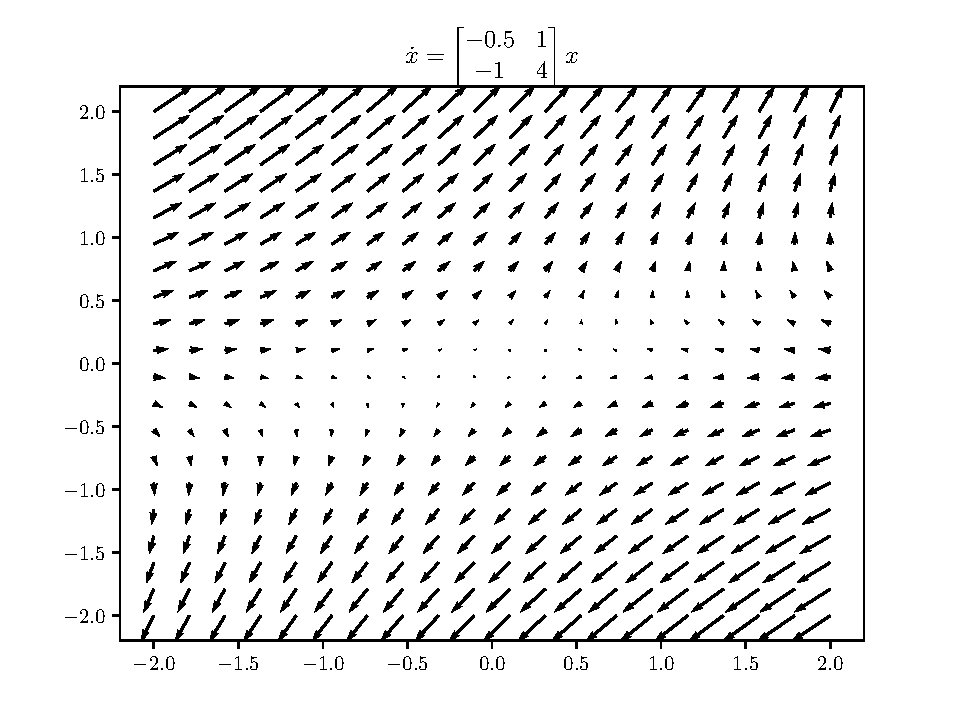
\includegraphics[scale=.75]{./tex/ch2/a.pdf}
        \caption{Vector field of a dynamic system.}
    \end{figure}
    \begin{figure}[H]
        \centering
        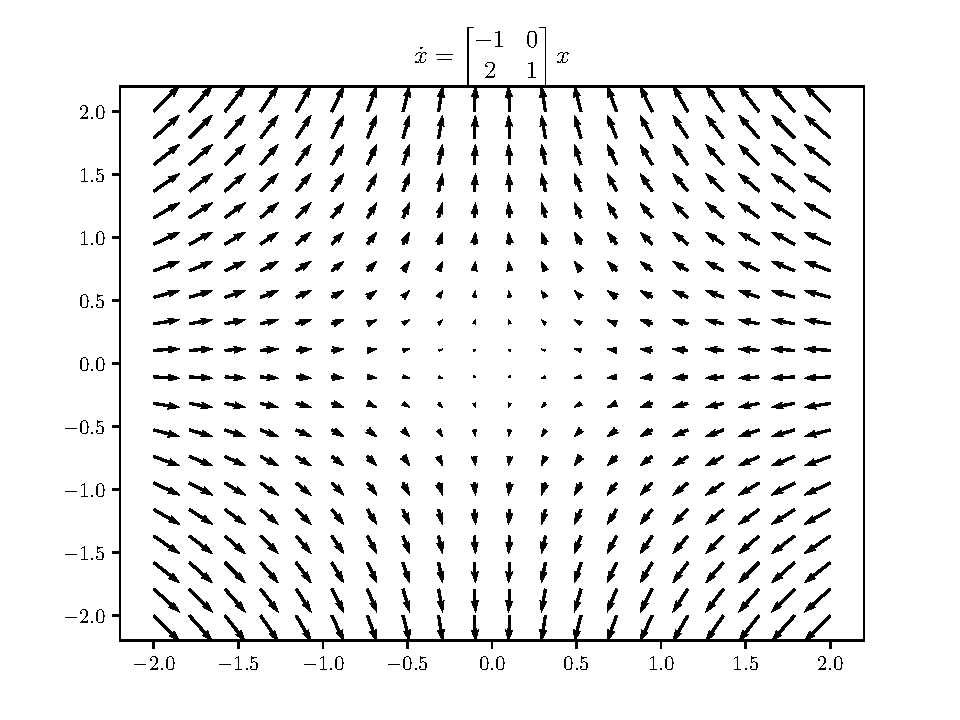
\includegraphics[scale=.75]{./tex/ch2/b.pdf}
        \caption{Vector field of another dynamic system.}
    \end{figure}
    \item Stability of continuous-time systems. $\dot x = Ax$ is stable if $\text{re}(\text{eigvals}(A))<0$,
    \item Solution to linear ODE (only one variable):
    \begin{equation}
        \dot{x} =ax\Rightarrow \frac{dx}{dt} =ax\Rightarrow \int \frac{1}{x} dx=\int adt\Rightarrow \ln x=at+C\Rightarrow x=e^{at+C} \Rightarrow x=e^{at} x_{0}
    \end{equation}
    \item Solution to linear ODE (multiple variable):
    \begin{equation}
        \dot{x} =Ax\Rightarrow e^{At} x_{0}
    \end{equation}
    \item Let us convert the above multi-variable continuous-time system to a discrete-time system:
    \begin{equation}
        x_{t+1}= \underbrace{e^{A\Delta t}}_{A_d} x_t
    \end{equation}
    \item Stability of discrete-time system: $\left|\text{eigvals}(A_d)\right|<1$,
    \item All the above is the autonomous system, now let us turn to control system. ZOH for control:
    \begin{equation}
        \begin{matrix}
        \dot{x} =Ax+Bu\\
        \dot{u} =0
        \end{matrix} \Rightarrow \begin{bmatrix}
        \dot{x}\\
        \dot{u}
        \end{bmatrix} =\begin{bmatrix}
        A & B\\
        0 & 0
        \end{bmatrix}\begin{bmatrix}
        x\\
        u
        \end{bmatrix} \qquad t\in\left(t_k, t_{k+1}\right), \text{this is another linear system}
    \end{equation}
    After discretization:
    \begin{equation}
        \begin{bmatrix}
        x_{k+1}\\
        u_{k+1}
        \end{bmatrix} =e^{\begin{bmatrix}
        A & B\\
        0 & 0
        \end{bmatrix} \Delta t}\begin{bmatrix}
        x_{t}\\
        u_{t}
        \end{bmatrix} \Rightarrow \begin{bmatrix}
        A_{d} & B_{d}\\
        0 & I
        \end{bmatrix} =e^{\begin{bmatrix}
        A & B\\
        0 & 0
        \end{bmatrix} \Delta t} \Rightarrow x_{t+1} =A_{d} x_{t} +B_{d} u_{t}
    \end{equation}
    \item Extension to $\dot x = Ax + Bu + d$:  
    \begin{equation}
        \begin{bmatrix}
        x_{t+1}\\
        u_{t+1}\\
        d_{t+1}
        \end{bmatrix} =e^{\begin{bmatrix}
        A & B & I\\
        0 & 0 & 0\\
        0 & 0 & 0
        \end{bmatrix} \Delta t}\begin{bmatrix}
        x_{t}\\
        u_{t}\\
        d_{t}
        \end{bmatrix} \Rightarrow \begin{bmatrix}
        A_{d} & B_{d} & D_{d}\\
        0 & I & 0\\
        0 & 0 & I
        \end{bmatrix} =e^{\begin{bmatrix}
        A & B & I\\
        0 & 0 & 0\\
        0 & 0 & 0
        \end{bmatrix} \Delta t} \Rightarrow x_{t+1} =A_{d} x_{t} +B_{d} u_{t} +D_{d} d_{t}
    \end{equation}
\subsection{Derivative Formalism}
Almost all the autodiff libraries use the same convention:
\begin{itemize}
    \item Jacobian: Given $f:\mathbb{R}^{N}\rightarrow \mathbb{R}^{M}$ (\verb|#| rows= \verb|#| outputs, \verb|#| cols= \verb|#| inputs):
    \begin{equation}
        \frac{\partial f}{\partial x} =\begin{bmatrix}
            \frac{\partial f_{1}}{\partial x_{1}} & \frac{\partial f_{1}}{\partial x_{2}} & \cdots  & \frac{\partial f_{1}}{\partial x_{N}}\\
            \frac{\partial f_{2}}{\partial x_{1}} & \frac{\partial f_{2}}{\partial x_{2}} & \cdots  & \frac{\partial f_{2}}{\partial x_{N}}\\
            \vdots  & \vdots  & \ddots  & \vdots \\
            \frac{\partial f_{M}}{\partial x_{1}} & \frac{\partial f_{M}}{\partial x_{2}} & \cdots  & \frac{\partial f_{M}}{\partial x_{N}}
        \end{bmatrix}
    \end{equation}
    \item Gradient: Given $f:\mathbb{R}^{N}\rightarrow \mathbb{R}$, be careful that $f$ must be a scalar valued function:
    \begin{equation}
        \frac{\partial f}{\partial x} =\begin{bmatrix}
            \frac{\partial f}{\partial x_{1}} & \frac{\partial f}{\partial x_{2}} & \cdots  & \frac{\partial f}{\partial x_{N}}
        \end{bmatrix} \qquad \text{, it is a row vector.}
    \end{equation}
    Just for convenient, we denote that:
    \begin{equation}
        \nabla_x f = \left(\frac{\partial f}{\partial x}\right)^T
    \end{equation}
    \item Hession: Given $f:\mathbb{R}^{N}\rightarrow \mathbb{R}$, be careful that $f$ must be a scalar valued function:
    \begin{equation}
        H = \ _x^2 f = \begin{bmatrix}
        \frac{\partial^2 f}{\partial x_1^2} & \frac{\partial^2 f}{\partial x_1 \partial x_2} & \cdots & \frac{\partial^2 f}{\partial x_1 \partial x_n} \\
        \frac{\partial^2 f}{\partial x_2 \partial x_1} & \frac{\partial^2 f}{\partial x_2^2} & \cdots & \frac{\partial^2 f}{\partial x_2 \partial x_n} \\
        \vdots & \vdots & \ddots & \vdots \\
        \frac{\partial^2 f}{\partial x_n \partial x_1} & \frac{\partial^2 f}{\partial x_n \partial x_2} & \cdots & \frac{\partial^2 f}{\partial x_n^2}
        \end{bmatrix} \qquad \text{, it is a symmetric matrix}
    \end{equation}
\end{itemize}
\subsection{Taylor Series}
For 1-input function:
\begin{equation}
    f(x) \approx f(a) + \frac{{\partial f}}{{\partial x}}\Bigg|_{x=a}(x - a)
\end{equation}
Normally, we denote that $x=a + \Delta x$:
\begin{equation}
    f(\bar x + \Delta x) \approx f(a) + \frac{{\partial f}}{{\partial x}}\Bigg|_{x=a}\Delta x
\end{equation}.
For 2-input function:
\begin{equation}
    f(x, y) \approx f(a, b) + \frac{{\partial f}}{{\partial x}}\Bigg|_{(a, b)}(x - a) + \frac{{\partial f}}{{\partial y}}\Bigg|_{(a, b)}(y - b)
\end{equation}
Normally, we denote that $x=a + \Delta x, y=b + \Delta y$:
\begin{equation}
    f(x, y) \approx f(a, b) + \frac{{\partial f}}{{\partial x}}\Bigg|_{(a, b)}\Delta x + \frac{{\partial f}}{{\partial y}}\Bigg|_{(a, b)}\Delta y
\end{equation}
\end{itemize}